\documentclass[12pt,doublespacing,a4paper]{ouparticle}

%\usepackage[scaled]{helvet}
%\renewcommand\familydefault{\sfdefault} 
%\usepackage[T1]{fontenc}

\usepackage[authoryear]{natbib}
\usepackage{lineno}
\usepackage{pdfpages}
\usepackage{lscape}

%\usepackage{enumerate}
\usepackage{enumitem} 

\usepackage{color}
\definecolor{darkgreen}{rgb}{0.0, 0.5, 0.0}
\definecolor{darkred}{rgb}{0.7, 0.11, 0.11}
\definecolor{darkblue}{rgb}{0,0,0.5}
\definecolor{shadecolor}{rgb}{1,1,0.95}
\definecolor{shade}{rgb}{1,1,0.95}
\definecolor{coilin}{rgb}{1,0,1}

\newcommand{\laurie}{\textcolor{red}}
\newcommand{\henning}{\textcolor{blue}}
\newcommand{\iago}{\textcolor{darkblue}}
\newcommand{\rishi}{\textcolor{darkred}}
\newcommand{\todo}[1]{\laurie{\textbf{\textit{#1}}}}

\begin{document}

\title{Non-Stationarity in Productivity.}

\author{%
\name{Laurence T. Kell 1, Rishi Sharma 2, Henning Winker 3, Toshihide Kitakado 4, Iago Mosqueira 5}
\address{1.Centre for Environmental Policy, Imperial College 2. FAO, Marine and Inland Fisheries, Rome, Italy 3. JRC, European Union, Ispra, Italy 4. Tokyo University of Marine Science and Technology, Tokyo, Japan 5. Waginengen University and Research, Netherlands  }
\email{e-mail Lauriel@seapluslus.co.uk}
\and
\name{}
\address{}
}

\abstract{
The Ecosystem Report Card of the Sub-Committee on Ecosystems includes indicators for assessed species  based on productivity, i.e. trends of biomass or spawning stock biomass relative and fishing mortality or harvest rate relative to Maximum Sustainable Yield reference points. The objective is to assess whether the main target stocks are in a healthy, cautious or critical state and how this has changed over time. Productivity, however, depends on physical and biological processes knowledge of which is important for ecosystem based fisheries management. We used the stock assessments for bigeye and yellowfin tunas from the Atlantic, Indian and Eastern Pacific Oceans, to illustrate the use of diagnostics based on production functions and surplus production verses biomass trajectories to explore changes in productivity.}

\date{\today}

\keywords{EBFM, productivity, bigeye, yellowfin}
 
\maketitle

\newpage


\linenumbers
\linespread{2}

\section{Introduction}

ICCAT has recently amended its Convention in order to move towards an Ecosystem Approach to Fisheries Management (EAFM). To do this the Commission and its Members shall act to: (a) apply the precautionary approach and an ecosystem approach to fisheries management in accordance with relevant internationally agreed standards and, as appropriate, recommended practices and procedures; (b) use the best scientific evidence available; and (c) protect biodiversity in the marine environment.

Currently the main tool developed by the SCRS to implement EAFM is the Ecosystem Report Card (ERC) of the Sub-Committee on Ecosystems (SC-ECO). This includes indicators for assessed species and as the Commission moves towards EAFM there is a need to develop models for stock assessment and management that integrate environmental conditions \citep{travis2014integrating}.  Particularly since growth and mortality, and recruitment, may be driven by environmental pressure.

Currently the indicators used for assessed species are based on the ratios of biomass or spawning stock biomass (SSB) relative to $B_{MSY}$, and fishing mortality or harvest rate relative to $F_{MSY}$. These indicators are obtained either from age-structured stock assessments that integrate changing vulnerability schedules, mean recruitment relationships, and recruitment anomalies, to estimate stock trends and reference points, or biomass dynamic assessments that fit a production function based on population growth rate ($r$), carrying capacity ($K$). In the age based models there is an implicit production function and process error is modelled either as variability in recruitment and/or selection pattern. In the biomass dynamic models with an explicit production function process error can be modelled explicitly.  

In age-structured models density dependence is mainly accounted for by the stock recruitment relationship. \cite{cury2014resolving}, however, showed that in most cases the stock-recruitment relationship used to estimate productivity and determine reference points, has poor estimation/predictive power and the environmental has a larger effect on productivity, a results confirmed by other studies \citep[e.g.][]{szuwalski2015examining, szuwalski2019global}(ADD Free, C.M., Thorson, J.T., Pinsky, M.L., Oken, K.L., Wiedenmann, J., Jensen, O.P., 2019. Impacts of historical warming on marine fisheries production. Sci 363, 979–983.) and observed 100 years ago by \cite{hjort1914fluctuations}. Whereas in ICCAT assessments growth, maturation and natural mortality are assumed not to have varied despite the large changes in the environment and stock biomass seen.

\cite{hilborn2001calculation} therefore recommended looking at patterns of change in surplus production (SP) since these may contain evidence of changes in the growth and mortality components of production, which are typically not represented in models currently used for stock assessment and management. 
%It is difficult, however, to examine empirical patterns in surplus production for the assessed ICCAT species since there is only limited fisheries independent data. An alternative is to estimate SP using assessment outputs. 
We therefore use the integrated stock assessments conducted with Stock Synthesis 3 (Methot and Wetzel 2013) \cite[SS3]{methot2005technical} for bigeye (in italics: Thunnus obesus) and yellowfin tuna (Thunnus albacares) stocks in the Atlantic, Indian and Eastern Pacific Oceans to estimate surplus production and explore whether the dynamics are determined by a production function or dynamics are recruitment-driven and influenced by the environment.

\section{Material and Methods}

\cite{walters2008surplus} argued that plotting of surplus production ($SP$) against biomass ($B$) should be one of the basic pieces of information presented in all stock assessments since the plots provide a check on whether there has been non-stationarity in the annual surplus production, i.e. whether similar $B$ levels have exhibited similar SP at different historical times. This is important for management as it checks whether predictions of changes in biomass ($B_{t+1} - B_t$) can be made reliably based on catch and $B_t$. Plots of $SP$ v $B$ therefore provide a summary of stock performance and include effects not necessarily included in stock assessment models. 

The effects not included in the production function used to predict $SP$ can be modelled by an process error term \epsilon$_t$.

$B_{t+1}=B_t-C_t+SP_t+\epsilon_t$
 
 Process error on biomass can account for model structural uncertainty as well as natural variability of stock biomass due to stochasticity in recruitment, natural mortality, growth, and maturation \citep{francis2011data} (add Meyer and Miller 1999; Winker et al. 2018).


%/ [HW: There are no results on this! Changes in recruitment and SPR 0 regimes were evaluated using a sequential t-test algorithm for regime shifts \citep{rodionov2004sequential}.

\begin{itemize}[topsep=0pt,itemsep=0ex,partopsep=0ex,parsep=0ex]
    %\item a direct check on whether predictions of changes in biomass ($B_{t+1} - B_t$) can be made reliably just based on catch and $B_t$, in particular whether similar $B$ levels have exhibited similar SP at different historical times, i.e., whether there has been non-stationarity in production processes. 
    %\item an overall summary of stock performance and include effects not necessarily included in stock assessment models. 
    %\item  a diagnostic for whether stocks have exhibited strong compensatory response, i.e., increase in $S/B$ at low stock sizes. Stocks that have not exhibited such responses have very likely been overfished over the whole period of historical record. In such cases reference points, e.g., $B_0$, should be viewed as highly speculative extrapolations that cannot be justified by available data, no matter how complex the stock assessment models used to analyze those data. 
    %\item  The plots are an important diagnostic for whether stock collapse has been due to overfishing or to antecedent decline in $S$ (that then caused $B$ to decline) attributable to factors other than stock size. 
    %\item ) While fitting SP curves to SP vs. B data is likely to result in highly biased estimates of unfished $B_{0}$, such fitting exercises are not expected to produce badly biased estimates of intrinsic population growth rate ro (Fmax) and hence of “good” target fishing mortality rates. As an example, F = $R_0/2$ is likely a good target exploitation rate that can be put in place without any reference to unfished stock size.
    %\item Note that we don't have the direction of the trajectory around the production function, i.e. it is clockwise its driven by the recruitment/pe and if its anticlockwise its driven by production function.
\end{itemize}

We therefore examine the relationships between surplus production and biomass  for bigeye and yellowfin tuna stocks in the Atlantic, Indian and Eastern Pacific Oceans using the results from integrated stock assessments. To do this we estimate annual surplus production as the change in stock size plus catch (i.e. $B_t – B_{t+1} + C_t$). We then plot the resulting time series of $S$ and $B$ to identify patterns of variation in $S$. 

The process error was then sampled from SS3 stock trajectories as the difference between deterministic expectation of biomass  and its stochastic realisation, such that:

\epsilon$_t = SB_t+1 - (SB_t+SP_t-C_t)$  (I'd prefer this on log-scale)

Long-term changes in process error regimes were evaluated using a sequential t-test algorithm for regime shifts \citep{rodionov2004sequential}.

 In the case of ICCAT and IOTC stocks, quarterly assessment models were used surplus production was calculated on an annual basis by aggregating catch and biomass across seasons and areas using r4ss\footnote{https://github.com/r4ss/r4ss}.
 
\section{Results}

Time series of SSB, biomass and catch relative to $MSY$ reference points are shown in \textbf{Figure} \ref{fig:ts}. For both ICCAT and IOTC stock has declined as a result of an increase in fishing pressure. In the case of ICCAT yellowfin a large increase in biomass and $SSB$ was seen which appears to have been independent of fishing pressure. The picture in the Eastern Pacific Ocean appears less clear as changes in biomass and $SSB$ appear to occur independently of fishing pressure.

Surplus production is plotted against biomass in \textbf{Figure} \ref{fig:sp}, dark to light colour of the trajectory indicates early to late periods. Clockwise cycling is seen in SP for IAATC bigeye, ICCAT yellowfin and IOTC yellowfin. This is caused by positive production anomalies, i.e. productivity over and above that predicted by the production function. 

The production functions, with trajectories of catch and biomass; red indicates region of overfishing and overfished, are shown in \textbf{Figure} \ref{fig:pf}.

%\textcolor{red}{Fig 3. ICCAT & IOTC stocks, quarterly models were used. Surplus was calculated in each quarterly step, but how? It multiplied 4 to compare with IATTC (?). Better to briefly explain how the curves were estimated in the text. Just in case, in theory, estimation of S-R after stock assessment needs consideration of errors-in-variables model, where data in x-y both axes have uncertainty, potentially a large variance.}

Time series of process error are shown in \textbf{Figure} \ref{fig:pe} and scaled relative to mean biomass, with regimes in \textbf{Figure} \ref{fig:pe2}. 

\section{Discussion}

ICCAT and IOTC stocks have shown long term declines, while both IATTC stocks have shown variability over time with no long term trend. This may be due to the model specification rather than the actual dynamics since IATTC uses a steepness value for the stock recruitment relationship (SSR) of h=0.99 which assumes that a means that dynamics are driven by recruitment, whereas ICCAT and IOTC use values in realms of 0.7-0.9.

The observed dynamics may also be an indication of model misspecification. Diagnostic tools to check for model mis-specification and validation currently includes  deterministic Age-Structured Production Model (ASPM), likelihood profiling (Maunder and Piner xxx) and Runs Tests (Maunder & Piner 2015; Carvalho et al. 2017), but need to be developed further, specifically with regards to implication for assessment model prediction skill under non-stationary process error (Kell et al. 2016; Chang et al. 2019).

Independent and positive lognormal recruitment anomalies resulted in pronounced clockwise loop of successive values when $SP_t$ is plotted against stock size $SB_t$ for IATTC bigeye, ICCAT yellowfin and IOTC yellowfin implying that dynamics are recruitment driven. For IOTC bigeye and yellowfin, larger values of $SP_t$ were seen at low stock biomass. 

 
%\cite{walters} showed that the usual assumptions in age-structured models (stable body growth, no change in natural mortality rate, recruitment following a Beverton–Holt curve) generally implies lower $S$ during population recoveries than during declines because of reduction in mean fecundity.

\section{Consequences for EBFM indicators}

In contrast Ecosystem models without age-structured effects typically predict the opposite pattern: higher SP at each stock size during recoveries than declines. Lower production during recoveries is often predicted by ecosystem models with size- and age-structured dynamics, especially when there are cultivation–depensation effects at play (Walters and Kitchell 2001, Liermann and Hilborn 1997). 

Higher production rates during recoveries are sometimes predicted by ecosystem models with size- and age-structure effects, but only when such models include ecosystem-scale changes in productivity (regime shifts), such that trophically driven increases in production can drive population increases/vice versa where we don't observe these increases as a function of these changes in the ecosystem, and hence we see lower production at lower biomass levels. 

Further, it has not been made clear what relationships we should expect between overall biomass and SP during population declines and recoveries and in particular whether age-structured and ecosystem models predict “non-stationarity” in the biomass–production relationship such that production rates exhibited at given biomass levels during recoveries might differ greatly from rates exhibited during declines. A particular concern is whether we should expect slower recoveries (lower SP at each stock size) than we would predict from production rates observed during declines, i.e., should populations recover more slowly than expected from simple dome-shaped production model theory (Hutchings and Reynolds 2004). For example, simulation studies have identified poor forecast performance when autocorrelation in recruitment was ignored (Johnson et al., 2016), which was associated with an increased risk of a “stochastic collapse” (Thorson et al., 2015).

In the Pacific Fishery Management Council (PFMC, Source , Citation), they use an age-structured model to predict recoveries so it would automatically incorporate at least recruitment effects caused by reduced mean fecundity in growing populations. Reduced mean fecundity in growing populations occurs because the population age structure is shifted toward younger fish, i.e., there is a proportional scarcity of older, more fecund individuals.

Here we examine observed relationships between SP rates and stock size for a variety of stocks. We estimate annual SP as change in stock size plus catch (SP = stock next year – stock this year + catch) and plot resulting empirical time series of SP and biomass estimates to look directly at patterns of variation in SP with biomass. We compare these patterns to those predicted by age-structured population models and by ecosystem models with and without age-structure effects. 

We show that the usual assumptions in age-structured models (stable body growth, no change in natural mortality rate, recruitment following Beverton–Holt curve on average) generally imply lower SP during population recoveries than during declines because of reduction in mean fecundity. However, independent lognormal recruitment anomalies cause the opposite effect, with each positive anomaly resulting in a clockwise loop of successive values when SP is plotted against stock size; further, such anomalies can cause severe bias in estimates of unfished stock size, when a simple SP curve is fitted to the production vs. biomass data. We show that ecosystem models without age-structured effects typically predict the opposite pattern: higher SP at each stock size during recoveries than declines. Lower production during recoveries is often predicted by ecosystem models with size- and age-structured dynamics, especially when there are cultivation–depensation effects at play (Walters and Kitchell 2001). 

Higher production rates during recoveries are sometimes predicted by ecosystem models with size- and age-structure effects, but only when such models include ecosystem-scale changes in productivity (regime shifts), such that trophically driven increases in production can drive population increases. We recommend that simple plots of SP rate vs. stock size be provided with stock assessment and ecosystem model results in general.

Winker et. al.(2020 jabbasel) noted that age-structured production models (ASPMs) are often preferred over biomass aggregated surplus production models (SPMs) as the former can track the propagation of cohorts and explicitly account for the effects of selective fishing, even in the absence of reliable size- or age data. ‘JABBA-Select’, an extension of the JABBA software (Just Another Bayesian Biomass Assessment; Winker et al., 2018), is able to overcome some of the shortcomings of conventional SPMs and allows a direct comparison to ASPMs. 

\begin{itemize}[labelindent=\parindent,noitemsep,topsep=0pt,parsep=0pt,partopsep=0pt]
\item Finally, the presence of clockwise cycling due to recruitment anomalies, implies that future catches are driven by incoming year classes, rather than the production function.
\item There appears to be a suggestion that the stock may be more productive at low stock size that predicted by the implicit production function and reference points derived from them.

Additional work would need to look at estimates of growth and mortality, e.g. from tagging studies, to assess why these production functions are clockwise in direction.

As suggested earlier, there is possibility of model mis-specification, as some of the commissions omit the possibility of a SSR by setting the default a recruitment driven stock (h=0.99 in IATTC), which may or may not be the case.

Operating Models used in MSE should be conditioned on hypotheses related to ecological processes, particularly as this study showed that either the models used for stock assessment are mis-specified or do not account for important ecological processes.

\end{itemize}


\section{Acknowledgement}


\clearpage
%\bibliography{/home/laurence-kell/Desktop/refs.bib}
%\bibliographystyle{apalike}
\documentclass[12pt,doublespacing,a4paper]{ouparticle}

%\usepackage[scaled]{helvet}
%\renewcommand\familydefault{\sfdefault} 
%\usepackage[T1]{fontenc}

\usepackage[authoryear]{natbib}
\usepackage{lineno}
\usepackage{pdfpages}
\usepackage{lscape}

%\usepackage{enumerate}
\usepackage{enumitem} 

\usepackage{color}
\definecolor{darkgreen}{rgb}{0.0, 0.5, 0.0}
\definecolor{darkred}{rgb}{0.7, 0.11, 0.11}
\definecolor{darkblue}{rgb}{0,0,0.5}
\definecolor{shadecolor}{rgb}{1,1,0.95}
\definecolor{shade}{rgb}{1,1,0.95}
\definecolor{coilin}{rgb}{1,0,1}

\newcommand{\laurie}{\textcolor{red}}
\newcommand{\henning}{\textcolor{blue}}
\newcommand{\iago}{\textcolor{darkblue}}
\newcommand{\rishi}{\textcolor{darkred}}
\newcommand{\todo}[1]{\laurie{\textbf{\textit{#1}}}}

\begin{document}

\title{Non-Stationarity in Productivity.}

\author{%
\name{Laurence T. Kell 1, Rishi Sharma 2, Henning Winker 3, Toshihide Kitakado 4, Iago Mosqueira 5}
\address{1.Centre for Environmental Policy, Imperial College 2. FAO, Marine and Inland Fisheries, Rome, Italy 3. JRC, European Union, Ispra, Italy 4. Tokyo University of Marine Science and Technology, Tokyo, Japan 5. Waginengen University and Research, Netherlands  }
\email{e-mail Lauriel@seapluslus.co.uk}
\and
\name{}
\address{}
}

\abstract{
The Ecosystem Report Card of the Sub-Committee on Ecosystems includes indicators for assessed species  based on productivity, i.e. trends of biomass or spawning stock biomass relative and fishing mortality or harvest rate relative to Maximum Sustainable Yield reference points. The objective is to assess whether the main target stocks are in a healthy, cautious or critical state and how this has changed over time. Productivity, however, depends on physical and biological processes knowledge of which is important for ecosystem based fisheries management. We used the stock assessments for bigeye and yellowfin tunas from the Atlantic, Indian and Eastern Pacific Oceans, to illustrate the use of diagnostics based on production functions and surplus production verses biomass trajectories to explore changes in productivity.}

\date{\today}

\keywords{EBFM, productivity, bigeye, yellowfin}
 
\maketitle

\newpage


\linenumbers
\linespread{2}

\section{Introduction}

ICCAT has recently amended its Convention in order to move towards an Ecosystem Approach to Fisheries Management (EAFM). To do this the Commission and its Members shall act to: (a) apply the precautionary approach and an ecosystem approach to fisheries management in accordance with relevant internationally agreed standards and, as appropriate, recommended practices and procedures; (b) use the best scientific evidence available; and (c) protect biodiversity in the marine environment.

Currently the main tool developed by the SCRS to implement EAFM is the Ecosystem Report Card (ERC) of the Sub-Committee on Ecosystems (SC-ECO). This includes indicators for assessed species and as the Commission moves towards EAFM there is a need to develop models for stock assessment and management that integrate environmental conditions \citep{travis2014integrating}.  Particularly since growth and mortality, and recruitment, may be driven by environmental pressure.

Currently the indicators used for assessed species are based on the ratios of biomass or spawning stock biomass (SSB) relative to $B_{MSY}$, and fishing mortality or harvest rate relative to $F_{MSY}$. These indicators are obtained either from age-structured stock assessments that integrate changing vulnerability schedules, mean recruitment relationships, and recruitment anomalies, to estimate stock trends and reference points, or biomass dynamic assessments that fit a production function based on population growth rate ($r$), carrying capacity ($K$). In the age based models there is an implicit production function and process error is modelled either as variability in recruitment and/or selection pattern. In the biomass dynamic models with an explicit production function process error can be modelled explicitly.  

In age-structured models density dependence is mainly accounted for by the stock recruitment relationship. \cite{cury2014resolving}, however, showed that in most cases the stock-recruitment relationship used to estimate productivity and determine reference points, has poor estimation/predictive power and the environmental has a larger effect on productivity, a results confirmed by other studies \citep[e.g.][]{szuwalski2015examining, szuwalski2019global}(ADD Free, C.M., Thorson, J.T., Pinsky, M.L., Oken, K.L., Wiedenmann, J., Jensen, O.P., 2019. Impacts of historical warming on marine fisheries production. Sci 363, 979–983.) and observed 100 years ago by \cite{hjort1914fluctuations}. Whereas in ICCAT assessments growth, maturation and natural mortality are assumed not to have varied despite the large changes in the environment and stock biomass seen.

\cite{hilborn2001calculation} therefore recommended looking at patterns of change in surplus production (SP) since these may contain evidence of changes in the growth and mortality components of production, which are typically not represented in models currently used for stock assessment and management. 
%It is difficult, however, to examine empirical patterns in surplus production for the assessed ICCAT species since there is only limited fisheries independent data. An alternative is to estimate SP using assessment outputs. 
We therefore use the integrated stock assessments conducted with Stock Synthesis 3 (Methot and Wetzel 2013) \cite[SS3]{methot2005technical} for bigeye (in italics: Thunnus obesus) and yellowfin tuna (Thunnus albacares) stocks in the Atlantic, Indian and Eastern Pacific Oceans to estimate surplus production and explore whether the dynamics are determined by a production function or dynamics are recruitment-driven and influenced by the environment.

\section{Material and Methods}

\cite{walters2008surplus} argued that plotting of surplus production ($SP$) against biomass ($B$) should be one of the basic pieces of information presented in all stock assessments since the plots provide a check on whether there has been non-stationarity in the annual surplus production, i.e. whether similar $B$ levels have exhibited similar SP at different historical times. This is important for management as it checks whether predictions of changes in biomass ($B_{t+1} - B_t$) can be made reliably based on catch and $B_t$. Plots of $SP$ v $B$ therefore provide a summary of stock performance and include effects not necessarily included in stock assessment models. 

The effects not included in the production function used to predict $SP$ can be modelled by an process error term \epsilon$_t$.

$B_{t+1}=B_t-C_t+SP_t+\epsilon_t$
 
 Process error on biomass can account for model structural uncertainty as well as natural variability of stock biomass due to stochasticity in recruitment, natural mortality, growth, and maturation \citep{francis2011data} (add Meyer and Miller 1999; Winker et al. 2018).


%/ [HW: There are no results on this! Changes in recruitment and SPR 0 regimes were evaluated using a sequential t-test algorithm for regime shifts \citep{rodionov2004sequential}.

\begin{itemize}[topsep=0pt,itemsep=0ex,partopsep=0ex,parsep=0ex]
    %\item a direct check on whether predictions of changes in biomass ($B_{t+1} - B_t$) can be made reliably just based on catch and $B_t$, in particular whether similar $B$ levels have exhibited similar SP at different historical times, i.e., whether there has been non-stationarity in production processes. 
    %\item an overall summary of stock performance and include effects not necessarily included in stock assessment models. 
    %\item  a diagnostic for whether stocks have exhibited strong compensatory response, i.e., increase in $S/B$ at low stock sizes. Stocks that have not exhibited such responses have very likely been overfished over the whole period of historical record. In such cases reference points, e.g., $B_0$, should be viewed as highly speculative extrapolations that cannot be justified by available data, no matter how complex the stock assessment models used to analyze those data. 
    %\item  The plots are an important diagnostic for whether stock collapse has been due to overfishing or to antecedent decline in $S$ (that then caused $B$ to decline) attributable to factors other than stock size. 
    %\item ) While fitting SP curves to SP vs. B data is likely to result in highly biased estimates of unfished $B_{0}$, such fitting exercises are not expected to produce badly biased estimates of intrinsic population growth rate ro (Fmax) and hence of “good” target fishing mortality rates. As an example, F = $R_0/2$ is likely a good target exploitation rate that can be put in place without any reference to unfished stock size.
    %\item Note that we don't have the direction of the trajectory around the production function, i.e. it is clockwise its driven by the recruitment/pe and if its anticlockwise its driven by production function.
\end{itemize}

We therefore examine the relationships between surplus production and biomass  for bigeye and yellowfin tuna stocks in the Atlantic, Indian and Eastern Pacific Oceans using the results from integrated stock assessments. To do this we estimate annual surplus production as the change in stock size plus catch (i.e. $B_t – B_{t+1} + C_t$). We then plot the resulting time series of $S$ and $B$ to identify patterns of variation in $S$. 

The process error was then sampled from SS3 stock trajectories as the difference between deterministic expectation of biomass  and its stochastic realisation, such that:

\epsilon$_t = SB_t+1 - (SB_t+SP_t-C_t)$  (I'd prefer this on log-scale)

Long-term changes in process error regimes were evaluated using a sequential t-test algorithm for regime shifts \citep{rodionov2004sequential}.

 In the case of ICCAT and IOTC stocks, quarterly assessment models were used surplus production was calculated on an annual basis by aggregating catch and biomass across seasons and areas using r4ss\footnote{https://github.com/r4ss/r4ss}.
 
\section{Results}

Time series of SSB, biomass and catch relative to $MSY$ reference points are shown in \textbf{Figure} \ref{fig:ts}. For both ICCAT and IOTC stock has declined as a result of an increase in fishing pressure. In the case of ICCAT yellowfin a large increase in biomass and $SSB$ was seen which appears to have been independent of fishing pressure. The picture in the Eastern Pacific Ocean appears less clear as changes in biomass and $SSB$ appear to occur independently of fishing pressure.

Surplus production is plotted against biomass in \textbf{Figure} \ref{fig:sp}, dark to light colour of the trajectory indicates early to late periods. Clockwise cycling is seen in SP for IAATC bigeye, ICCAT yellowfin and IOTC yellowfin. This is caused by positive production anomalies, i.e. productivity over and above that predicted by the production function. 

The production functions, with trajectories of catch and biomass; red indicates region of overfishing and overfished, are shown in \textbf{Figure} \ref{fig:pf}.

%\textcolor{red}{Fig 3. ICCAT & IOTC stocks, quarterly models were used. Surplus was calculated in each quarterly step, but how? It multiplied 4 to compare with IATTC (?). Better to briefly explain how the curves were estimated in the text. Just in case, in theory, estimation of S-R after stock assessment needs consideration of errors-in-variables model, where data in x-y both axes have uncertainty, potentially a large variance.}

Time series of process error are shown in \textbf{Figure} \ref{fig:pe} and scaled relative to mean biomass, with regimes in \textbf{Figure} \ref{fig:pe2}. 

\section{Discussion}

ICCAT and IOTC stocks have shown long term declines, while both IATTC stocks have shown variability over time with no long term trend. This may be due to the model specification rather than the actual dynamics since IATTC uses a steepness value for the stock recruitment relationship (SSR) of h=0.99 which assumes that a means that dynamics are driven by recruitment, whereas ICCAT and IOTC use values in realms of 0.7-0.9.

The observed dynamics may also be an indication of model misspecification. Diagnostic tools to check for model mis-specification and validation currently includes  deterministic Age-Structured Production Model (ASPM), likelihood profiling (Maunder and Piner xxx) and Runs Tests (Maunder & Piner 2015; Carvalho et al. 2017), but need to be developed further, specifically with regards to implication for assessment model prediction skill under non-stationary process error (Kell et al. 2016; Chang et al. 2019).

Independent and positive lognormal recruitment anomalies resulted in pronounced clockwise loop of successive values when $SP_t$ is plotted against stock size $SB_t$ for IATTC bigeye, ICCAT yellowfin and IOTC yellowfin implying that dynamics are recruitment driven. For IOTC bigeye and yellowfin, larger values of $SP_t$ were seen at low stock biomass. 

 
%\cite{walters} showed that the usual assumptions in age-structured models (stable body growth, no change in natural mortality rate, recruitment following a Beverton–Holt curve) generally implies lower $S$ during population recoveries than during declines because of reduction in mean fecundity.

\section{Consequences for EBFM indicators}

In contrast Ecosystem models without age-structured effects typically predict the opposite pattern: higher SP at each stock size during recoveries than declines. Lower production during recoveries is often predicted by ecosystem models with size- and age-structured dynamics, especially when there are cultivation–depensation effects at play (Walters and Kitchell 2001, Liermann and Hilborn 1997). 

Higher production rates during recoveries are sometimes predicted by ecosystem models with size- and age-structure effects, but only when such models include ecosystem-scale changes in productivity (regime shifts), such that trophically driven increases in production can drive population increases/vice versa where we don't observe these increases as a function of these changes in the ecosystem, and hence we see lower production at lower biomass levels. 

Further, it has not been made clear what relationships we should expect between overall biomass and SP during population declines and recoveries and in particular whether age-structured and ecosystem models predict “non-stationarity” in the biomass–production relationship such that production rates exhibited at given biomass levels during recoveries might differ greatly from rates exhibited during declines. A particular concern is whether we should expect slower recoveries (lower SP at each stock size) than we would predict from production rates observed during declines, i.e., should populations recover more slowly than expected from simple dome-shaped production model theory (Hutchings and Reynolds 2004). For example, simulation studies have identified poor forecast performance when autocorrelation in recruitment was ignored (Johnson et al., 2016), which was associated with an increased risk of a “stochastic collapse” (Thorson et al., 2015).

In the Pacific Fishery Management Council (PFMC, Source , Citation), they use an age-structured model to predict recoveries so it would automatically incorporate at least recruitment effects caused by reduced mean fecundity in growing populations. Reduced mean fecundity in growing populations occurs because the population age structure is shifted toward younger fish, i.e., there is a proportional scarcity of older, more fecund individuals.

Here we examine observed relationships between SP rates and stock size for a variety of stocks. We estimate annual SP as change in stock size plus catch (SP = stock next year – stock this year + catch) and plot resulting empirical time series of SP and biomass estimates to look directly at patterns of variation in SP with biomass. We compare these patterns to those predicted by age-structured population models and by ecosystem models with and without age-structure effects. 

We show that the usual assumptions in age-structured models (stable body growth, no change in natural mortality rate, recruitment following Beverton–Holt curve on average) generally imply lower SP during population recoveries than during declines because of reduction in mean fecundity. However, independent lognormal recruitment anomalies cause the opposite effect, with each positive anomaly resulting in a clockwise loop of successive values when SP is plotted against stock size; further, such anomalies can cause severe bias in estimates of unfished stock size, when a simple SP curve is fitted to the production vs. biomass data. We show that ecosystem models without age-structured effects typically predict the opposite pattern: higher SP at each stock size during recoveries than declines. Lower production during recoveries is often predicted by ecosystem models with size- and age-structured dynamics, especially when there are cultivation–depensation effects at play (Walters and Kitchell 2001). 

Higher production rates during recoveries are sometimes predicted by ecosystem models with size- and age-structure effects, but only when such models include ecosystem-scale changes in productivity (regime shifts), such that trophically driven increases in production can drive population increases. We recommend that simple plots of SP rate vs. stock size be provided with stock assessment and ecosystem model results in general.

Winker et. al.(2020 jabbasel) noted that age-structured production models (ASPMs) are often preferred over biomass aggregated surplus production models (SPMs) as the former can track the propagation of cohorts and explicitly account for the effects of selective fishing, even in the absence of reliable size- or age data. ‘JABBA-Select’, an extension of the JABBA software (Just Another Bayesian Biomass Assessment; Winker et al., 2018), is able to overcome some of the shortcomings of conventional SPMs and allows a direct comparison to ASPMs. 

\begin{itemize}[labelindent=\parindent,noitemsep,topsep=0pt,parsep=0pt,partopsep=0pt]
\item Finally, the presence of clockwise cycling due to recruitment anomalies, implies that future catches are driven by incoming year classes, rather than the production function.
\item There appears to be a suggestion that the stock may be more productive at low stock size that predicted by the implicit production function and reference points derived from them.

Additional work would need to look at estimates of growth and mortality, e.g. from tagging studies, to assess why these production functions are clockwise in direction.

As suggested earlier, there is possibility of model mis-specification, as some of the commissions omit the possibility of a SSR by setting the default a recruitment driven stock (h=0.99 in IATTC), which may or may not be the case.

Operating Models used in MSE should be conditioned on hypotheses related to ecological processes, particularly as this study showed that either the models used for stock assessment are mis-specified or do not account for important ecological processes.

\end{itemize}


\section{Acknowledgement}


\clearpage
%\bibliography{/home/laurence-kell/Desktop/refs.bib}
%\bibliographystyle{apalike}
\documentclass[12pt,doublespacing,a4paper]{ouparticle}

%\usepackage[scaled]{helvet}
%\renewcommand\familydefault{\sfdefault} 
%\usepackage[T1]{fontenc}

\usepackage[authoryear]{natbib}
\usepackage{lineno}
\usepackage{pdfpages}
\usepackage{lscape}

%\usepackage{enumerate}
\usepackage{enumitem} 

\usepackage{color}
\definecolor{darkgreen}{rgb}{0.0, 0.5, 0.0}
\definecolor{darkred}{rgb}{0.7, 0.11, 0.11}
\definecolor{darkblue}{rgb}{0,0,0.5}
\definecolor{shadecolor}{rgb}{1,1,0.95}
\definecolor{shade}{rgb}{1,1,0.95}
\definecolor{coilin}{rgb}{1,0,1}

\newcommand{\laurie}{\textcolor{red}}
\newcommand{\henning}{\textcolor{blue}}
\newcommand{\iago}{\textcolor{darkblue}}
\newcommand{\rishi}{\textcolor{darkred}}
\newcommand{\todo}[1]{\laurie{\textbf{\textit{#1}}}}

\begin{document}

\title{Non-Stationarity in Productivity.}

\author{%
\name{Laurence T. Kell 1, Rishi Sharma 2, Henning Winker 3, Toshihide Kitakado 4, Iago Mosqueira 5}
\address{1.Centre for Environmental Policy, Imperial College 2. FAO, Marine and Inland Fisheries, Rome, Italy 3. JRC, European Union, Ispra, Italy 4. Tokyo University of Marine Science and Technology, Tokyo, Japan 5. Waginengen University and Research, Netherlands  }
\email{e-mail Lauriel@seapluslus.co.uk}
\and
\name{}
\address{}
}

\abstract{
The Ecosystem Report Card of the Sub-Committee on Ecosystems includes indicators for assessed species  based on productivity, i.e. trends of biomass or spawning stock biomass relative and fishing mortality or harvest rate relative to Maximum Sustainable Yield reference points. The objective is to assess whether the main target stocks are in a healthy, cautious or critical state and how this has changed over time. Productivity, however, depends on physical and biological processes knowledge of which is important for ecosystem based fisheries management. We used the stock assessments for bigeye and yellowfin tunas from the Atlantic, Indian and Eastern Pacific Oceans, to illustrate the use of diagnostics based on production functions and surplus production verses biomass trajectories to explore changes in productivity.}

\date{\today}

\keywords{EBFM, productivity, bigeye, yellowfin}
 
\maketitle

\newpage


\linenumbers
\linespread{2}

\section{Introduction}

ICCAT has recently amended its Convention in order to move towards an Ecosystem Approach to Fisheries Management (EAFM). To do this the Commission and its Members shall act to: (a) apply the precautionary approach and an ecosystem approach to fisheries management in accordance with relevant internationally agreed standards and, as appropriate, recommended practices and procedures; (b) use the best scientific evidence available; and (c) protect biodiversity in the marine environment.

Currently the main tool developed by the SCRS to implement EAFM is the Ecosystem Report Card (ERC) of the Sub-Committee on Ecosystems (SC-ECO). This includes indicators for assessed species and as the Commission moves towards EAFM there is a need to develop models for stock assessment and management that integrate environmental conditions \citep{travis2014integrating}.  Particularly since growth and mortality, and recruitment, may be driven by environmental pressure.

Currently the indicators used for assessed species are based on the ratios of biomass or spawning stock biomass (SSB) relative to $B_{MSY}$, and fishing mortality or harvest rate relative to $F_{MSY}$. These indicators are obtained either from age-structured stock assessments that integrate changing vulnerability schedules, mean recruitment relationships, and recruitment anomalies, to estimate stock trends and reference points, or biomass dynamic assessments that fit a production function based on population growth rate ($r$), carrying capacity ($K$). In the age based models there is an implicit production function and process error is modelled either as variability in recruitment and/or selection pattern. In the biomass dynamic models with an explicit production function process error can be modelled explicitly.  

In age-structured models density dependence is mainly accounted for by the stock recruitment relationship. \cite{cury2014resolving}, however, showed that in most cases the stock-recruitment relationship used to estimate productivity and determine reference points, has poor estimation/predictive power and the environmental has a larger effect on productivity, a results confirmed by other studies \citep[e.g.][]{szuwalski2015examining, szuwalski2019global}(ADD Free, C.M., Thorson, J.T., Pinsky, M.L., Oken, K.L., Wiedenmann, J., Jensen, O.P., 2019. Impacts of historical warming on marine fisheries production. Sci 363, 979–983.) and observed 100 years ago by \cite{hjort1914fluctuations}. Whereas in ICCAT assessments growth, maturation and natural mortality are assumed not to have varied despite the large changes in the environment and stock biomass seen.

\cite{hilborn2001calculation} therefore recommended looking at patterns of change in surplus production (SP) since these may contain evidence of changes in the growth and mortality components of production, which are typically not represented in models currently used for stock assessment and management. 
%It is difficult, however, to examine empirical patterns in surplus production for the assessed ICCAT species since there is only limited fisheries independent data. An alternative is to estimate SP using assessment outputs. 
We therefore use the integrated stock assessments conducted with Stock Synthesis 3 (Methot and Wetzel 2013) \cite[SS3]{methot2005technical} for bigeye (in italics: Thunnus obesus) and yellowfin tuna (Thunnus albacares) stocks in the Atlantic, Indian and Eastern Pacific Oceans to estimate surplus production and explore whether the dynamics are determined by a production function or dynamics are recruitment-driven and influenced by the environment.

\section{Material and Methods}

\cite{walters2008surplus} argued that plotting of surplus production ($SP$) against biomass ($B$) should be one of the basic pieces of information presented in all stock assessments since the plots provide a check on whether there has been non-stationarity in the annual surplus production, i.e. whether similar $B$ levels have exhibited similar SP at different historical times. This is important for management as it checks whether predictions of changes in biomass ($B_{t+1} - B_t$) can be made reliably based on catch and $B_t$. Plots of $SP$ v $B$ therefore provide a summary of stock performance and include effects not necessarily included in stock assessment models. 

The effects not included in the production function used to predict $SP$ can be modelled by an process error term \epsilon$_t$.

$B_{t+1}=B_t-C_t+SP_t+\epsilon_t$
 
 Process error on biomass can account for model structural uncertainty as well as natural variability of stock biomass due to stochasticity in recruitment, natural mortality, growth, and maturation \citep{francis2011data} (add Meyer and Miller 1999; Winker et al. 2018).


%/ [HW: There are no results on this! Changes in recruitment and SPR 0 regimes were evaluated using a sequential t-test algorithm for regime shifts \citep{rodionov2004sequential}.

\begin{itemize}[topsep=0pt,itemsep=0ex,partopsep=0ex,parsep=0ex]
    %\item a direct check on whether predictions of changes in biomass ($B_{t+1} - B_t$) can be made reliably just based on catch and $B_t$, in particular whether similar $B$ levels have exhibited similar SP at different historical times, i.e., whether there has been non-stationarity in production processes. 
    %\item an overall summary of stock performance and include effects not necessarily included in stock assessment models. 
    %\item  a diagnostic for whether stocks have exhibited strong compensatory response, i.e., increase in $S/B$ at low stock sizes. Stocks that have not exhibited such responses have very likely been overfished over the whole period of historical record. In such cases reference points, e.g., $B_0$, should be viewed as highly speculative extrapolations that cannot be justified by available data, no matter how complex the stock assessment models used to analyze those data. 
    %\item  The plots are an important diagnostic for whether stock collapse has been due to overfishing or to antecedent decline in $S$ (that then caused $B$ to decline) attributable to factors other than stock size. 
    %\item ) While fitting SP curves to SP vs. B data is likely to result in highly biased estimates of unfished $B_{0}$, such fitting exercises are not expected to produce badly biased estimates of intrinsic population growth rate ro (Fmax) and hence of “good” target fishing mortality rates. As an example, F = $R_0/2$ is likely a good target exploitation rate that can be put in place without any reference to unfished stock size.
    %\item Note that we don't have the direction of the trajectory around the production function, i.e. it is clockwise its driven by the recruitment/pe and if its anticlockwise its driven by production function.
\end{itemize}

We therefore examine the relationships between surplus production and biomass  for bigeye and yellowfin tuna stocks in the Atlantic, Indian and Eastern Pacific Oceans using the results from integrated stock assessments. To do this we estimate annual surplus production as the change in stock size plus catch (i.e. $B_t – B_{t+1} + C_t$). We then plot the resulting time series of $S$ and $B$ to identify patterns of variation in $S$. 

The process error was then sampled from SS3 stock trajectories as the difference between deterministic expectation of biomass  and its stochastic realisation, such that:

\epsilon$_t = SB_t+1 - (SB_t+SP_t-C_t)$  (I'd prefer this on log-scale)

Long-term changes in process error regimes were evaluated using a sequential t-test algorithm for regime shifts \citep{rodionov2004sequential}.

 In the case of ICCAT and IOTC stocks, quarterly assessment models were used surplus production was calculated on an annual basis by aggregating catch and biomass across seasons and areas using r4ss\footnote{https://github.com/r4ss/r4ss}.
 
\section{Results}

Time series of SSB, biomass and catch relative to $MSY$ reference points are shown in \textbf{Figure} \ref{fig:ts}. For both ICCAT and IOTC stock has declined as a result of an increase in fishing pressure. In the case of ICCAT yellowfin a large increase in biomass and $SSB$ was seen which appears to have been independent of fishing pressure. The picture in the Eastern Pacific Ocean appears less clear as changes in biomass and $SSB$ appear to occur independently of fishing pressure.

Surplus production is plotted against biomass in \textbf{Figure} \ref{fig:sp}, dark to light colour of the trajectory indicates early to late periods. Clockwise cycling is seen in SP for IAATC bigeye, ICCAT yellowfin and IOTC yellowfin. This is caused by positive production anomalies, i.e. productivity over and above that predicted by the production function. 

The production functions, with trajectories of catch and biomass; red indicates region of overfishing and overfished, are shown in \textbf{Figure} \ref{fig:pf}.

%\textcolor{red}{Fig 3. ICCAT & IOTC stocks, quarterly models were used. Surplus was calculated in each quarterly step, but how? It multiplied 4 to compare with IATTC (?). Better to briefly explain how the curves were estimated in the text. Just in case, in theory, estimation of S-R after stock assessment needs consideration of errors-in-variables model, where data in x-y both axes have uncertainty, potentially a large variance.}

Time series of process error are shown in \textbf{Figure} \ref{fig:pe} and scaled relative to mean biomass, with regimes in \textbf{Figure} \ref{fig:pe2}. 

\section{Discussion}

ICCAT and IOTC stocks have shown long term declines, while both IATTC stocks have shown variability over time with no long term trend. This may be due to the model specification rather than the actual dynamics since IATTC uses a steepness value for the stock recruitment relationship (SSR) of h=0.99 which assumes that a means that dynamics are driven by recruitment, whereas ICCAT and IOTC use values in realms of 0.7-0.9.

The observed dynamics may also be an indication of model misspecification. Diagnostic tools to check for model mis-specification and validation currently includes  deterministic Age-Structured Production Model (ASPM), likelihood profiling (Maunder and Piner xxx) and Runs Tests (Maunder & Piner 2015; Carvalho et al. 2017), but need to be developed further, specifically with regards to implication for assessment model prediction skill under non-stationary process error (Kell et al. 2016; Chang et al. 2019).

Independent and positive lognormal recruitment anomalies resulted in pronounced clockwise loop of successive values when $SP_t$ is plotted against stock size $SB_t$ for IATTC bigeye, ICCAT yellowfin and IOTC yellowfin implying that dynamics are recruitment driven. For IOTC bigeye and yellowfin, larger values of $SP_t$ were seen at low stock biomass. 

 
%\cite{walters} showed that the usual assumptions in age-structured models (stable body growth, no change in natural mortality rate, recruitment following a Beverton–Holt curve) generally implies lower $S$ during population recoveries than during declines because of reduction in mean fecundity.

\section{Consequences for EBFM indicators}

In contrast Ecosystem models without age-structured effects typically predict the opposite pattern: higher SP at each stock size during recoveries than declines. Lower production during recoveries is often predicted by ecosystem models with size- and age-structured dynamics, especially when there are cultivation–depensation effects at play (Walters and Kitchell 2001, Liermann and Hilborn 1997). 

Higher production rates during recoveries are sometimes predicted by ecosystem models with size- and age-structure effects, but only when such models include ecosystem-scale changes in productivity (regime shifts), such that trophically driven increases in production can drive population increases/vice versa where we don't observe these increases as a function of these changes in the ecosystem, and hence we see lower production at lower biomass levels. 

Further, it has not been made clear what relationships we should expect between overall biomass and SP during population declines and recoveries and in particular whether age-structured and ecosystem models predict “non-stationarity” in the biomass–production relationship such that production rates exhibited at given biomass levels during recoveries might differ greatly from rates exhibited during declines. A particular concern is whether we should expect slower recoveries (lower SP at each stock size) than we would predict from production rates observed during declines, i.e., should populations recover more slowly than expected from simple dome-shaped production model theory (Hutchings and Reynolds 2004). For example, simulation studies have identified poor forecast performance when autocorrelation in recruitment was ignored (Johnson et al., 2016), which was associated with an increased risk of a “stochastic collapse” (Thorson et al., 2015).

In the Pacific Fishery Management Council (PFMC, Source , Citation), they use an age-structured model to predict recoveries so it would automatically incorporate at least recruitment effects caused by reduced mean fecundity in growing populations. Reduced mean fecundity in growing populations occurs because the population age structure is shifted toward younger fish, i.e., there is a proportional scarcity of older, more fecund individuals.

Here we examine observed relationships between SP rates and stock size for a variety of stocks. We estimate annual SP as change in stock size plus catch (SP = stock next year – stock this year + catch) and plot resulting empirical time series of SP and biomass estimates to look directly at patterns of variation in SP with biomass. We compare these patterns to those predicted by age-structured population models and by ecosystem models with and without age-structure effects. 

We show that the usual assumptions in age-structured models (stable body growth, no change in natural mortality rate, recruitment following Beverton–Holt curve on average) generally imply lower SP during population recoveries than during declines because of reduction in mean fecundity. However, independent lognormal recruitment anomalies cause the opposite effect, with each positive anomaly resulting in a clockwise loop of successive values when SP is plotted against stock size; further, such anomalies can cause severe bias in estimates of unfished stock size, when a simple SP curve is fitted to the production vs. biomass data. We show that ecosystem models without age-structured effects typically predict the opposite pattern: higher SP at each stock size during recoveries than declines. Lower production during recoveries is often predicted by ecosystem models with size- and age-structured dynamics, especially when there are cultivation–depensation effects at play (Walters and Kitchell 2001). 

Higher production rates during recoveries are sometimes predicted by ecosystem models with size- and age-structure effects, but only when such models include ecosystem-scale changes in productivity (regime shifts), such that trophically driven increases in production can drive population increases. We recommend that simple plots of SP rate vs. stock size be provided with stock assessment and ecosystem model results in general.

Winker et. al.(2020 jabbasel) noted that age-structured production models (ASPMs) are often preferred over biomass aggregated surplus production models (SPMs) as the former can track the propagation of cohorts and explicitly account for the effects of selective fishing, even in the absence of reliable size- or age data. ‘JABBA-Select’, an extension of the JABBA software (Just Another Bayesian Biomass Assessment; Winker et al., 2018), is able to overcome some of the shortcomings of conventional SPMs and allows a direct comparison to ASPMs. 

\begin{itemize}[labelindent=\parindent,noitemsep,topsep=0pt,parsep=0pt,partopsep=0pt]
\item Finally, the presence of clockwise cycling due to recruitment anomalies, implies that future catches are driven by incoming year classes, rather than the production function.
\item There appears to be a suggestion that the stock may be more productive at low stock size that predicted by the implicit production function and reference points derived from them.

Additional work would need to look at estimates of growth and mortality, e.g. from tagging studies, to assess why these production functions are clockwise in direction.

As suggested earlier, there is possibility of model mis-specification, as some of the commissions omit the possibility of a SSR by setting the default a recruitment driven stock (h=0.99 in IATTC), which may or may not be the case.

Operating Models used in MSE should be conditioned on hypotheses related to ecological processes, particularly as this study showed that either the models used for stock assessment are mis-specified or do not account for important ecological processes.

\end{itemize}


\section{Acknowledgement}


\clearpage
%\bibliography{/home/laurence-kell/Desktop/refs.bib}
%\bibliographystyle{apalike}
\documentclass[12pt,doublespacing,a4paper]{ouparticle}

%\usepackage[scaled]{helvet}
%\renewcommand\familydefault{\sfdefault} 
%\usepackage[T1]{fontenc}

\usepackage[authoryear]{natbib}
\usepackage{lineno}
\usepackage{pdfpages}
\usepackage{lscape}

%\usepackage{enumerate}
\usepackage{enumitem} 

\usepackage{color}
\definecolor{darkgreen}{rgb}{0.0, 0.5, 0.0}
\definecolor{darkred}{rgb}{0.7, 0.11, 0.11}
\definecolor{darkblue}{rgb}{0,0,0.5}
\definecolor{shadecolor}{rgb}{1,1,0.95}
\definecolor{shade}{rgb}{1,1,0.95}
\definecolor{coilin}{rgb}{1,0,1}

\newcommand{\laurie}{\textcolor{red}}
\newcommand{\henning}{\textcolor{blue}}
\newcommand{\iago}{\textcolor{darkblue}}
\newcommand{\rishi}{\textcolor{darkred}}
\newcommand{\todo}[1]{\laurie{\textbf{\textit{#1}}}}

\begin{document}

\title{Non-Stationarity in Productivity.}

\author{%
\name{Laurence T. Kell 1, Rishi Sharma 2, Henning Winker 3, Toshihide Kitakado 4, Iago Mosqueira 5}
\address{1.Centre for Environmental Policy, Imperial College 2. FAO, Marine and Inland Fisheries, Rome, Italy 3. JRC, European Union, Ispra, Italy 4. Tokyo University of Marine Science and Technology, Tokyo, Japan 5. Waginengen University and Research, Netherlands  }
\email{e-mail Lauriel@seapluslus.co.uk}
\and
\name{}
\address{}
}

\abstract{
The Ecosystem Report Card of the Sub-Committee on Ecosystems includes indicators for assessed species  based on productivity, i.e. trends of biomass or spawning stock biomass relative and fishing mortality or harvest rate relative to Maximum Sustainable Yield reference points. The objective is to assess whether the main target stocks are in a healthy, cautious or critical state and how this has changed over time. Productivity, however, depends on physical and biological processes knowledge of which is important for ecosystem based fisheries management. We used the stock assessments for bigeye and yellowfin tunas from the Atlantic, Indian and Eastern Pacific Oceans, to illustrate the use of diagnostics based on production functions and surplus production verses biomass trajectories to explore changes in productivity.}

\date{\today}

\keywords{EBFM, productivity, bigeye, yellowfin}
 
\maketitle

\newpage


\linenumbers
\linespread{2}

\section{Introduction}

ICCAT has recently amended its Convention in order to move towards an Ecosystem Approach to Fisheries Management (EAFM). To do this the Commission and its Members shall act to: (a) apply the precautionary approach and an ecosystem approach to fisheries management in accordance with relevant internationally agreed standards and, as appropriate, recommended practices and procedures; (b) use the best scientific evidence available; and (c) protect biodiversity in the marine environment.

Currently the main tool developed by the SCRS to implement EAFM is the Ecosystem Report Card (ERC) of the Sub-Committee on Ecosystems (SC-ECO). This includes indicators for assessed species and as the Commission moves towards EAFM there is a need to develop models for stock assessment and management that integrate environmental conditions \citep{travis2014integrating}.  Particularly since growth and mortality, and recruitment, may be driven by environmental pressure.

Currently the indicators used for assessed species are based on the ratios of biomass or spawning stock biomass (SSB) relative to $B_{MSY}$, and fishing mortality or harvest rate relative to $F_{MSY}$. These indicators are obtained either from age-structured stock assessments that integrate changing vulnerability schedules, mean recruitment relationships, and recruitment anomalies, to estimate stock trends and reference points, or biomass dynamic assessments that fit a production function based on population growth rate ($r$), carrying capacity ($K$). In the age based models there is an implicit production function and process error is modelled either as variability in recruitment and/or selection pattern. In the biomass dynamic models with an explicit production function process error can be modelled explicitly.  

In age-structured models density dependence is mainly accounted for by the stock recruitment relationship. \cite{cury2014resolving}, however, showed that in most cases the stock-recruitment relationship used to estimate productivity and determine reference points, has poor estimation/predictive power and the environmental has a larger effect on productivity, a results confirmed by other studies \citep[e.g.][]{szuwalski2015examining, szuwalski2019global}(ADD Free, C.M., Thorson, J.T., Pinsky, M.L., Oken, K.L., Wiedenmann, J., Jensen, O.P., 2019. Impacts of historical warming on marine fisheries production. Sci 363, 979–983.) and observed 100 years ago by \cite{hjort1914fluctuations}. Whereas in ICCAT assessments growth, maturation and natural mortality are assumed not to have varied despite the large changes in the environment and stock biomass seen.

\cite{hilborn2001calculation} therefore recommended looking at patterns of change in surplus production (SP) since these may contain evidence of changes in the growth and mortality components of production, which are typically not represented in models currently used for stock assessment and management. 
%It is difficult, however, to examine empirical patterns in surplus production for the assessed ICCAT species since there is only limited fisheries independent data. An alternative is to estimate SP using assessment outputs. 
We therefore use the integrated stock assessments conducted with Stock Synthesis 3 (Methot and Wetzel 2013) \cite[SS3]{methot2005technical} for bigeye (in italics: Thunnus obesus) and yellowfin tuna (Thunnus albacares) stocks in the Atlantic, Indian and Eastern Pacific Oceans to estimate surplus production and explore whether the dynamics are determined by a production function or dynamics are recruitment-driven and influenced by the environment.

\section{Material and Methods}

\cite{walters2008surplus} argued that plotting of surplus production ($SP$) against biomass ($B$) should be one of the basic pieces of information presented in all stock assessments since the plots provide a check on whether there has been non-stationarity in the annual surplus production, i.e. whether similar $B$ levels have exhibited similar SP at different historical times. This is important for management as it checks whether predictions of changes in biomass ($B_{t+1} - B_t$) can be made reliably based on catch and $B_t$. Plots of $SP$ v $B$ therefore provide a summary of stock performance and include effects not necessarily included in stock assessment models. 

The effects not included in the production function used to predict $SP$ can be modelled by an process error term \epsilon$_t$.

$B_{t+1}=B_t-C_t+SP_t+\epsilon_t$
 
 Process error on biomass can account for model structural uncertainty as well as natural variability of stock biomass due to stochasticity in recruitment, natural mortality, growth, and maturation \citep{francis2011data} (add Meyer and Miller 1999; Winker et al. 2018).


%/ [HW: There are no results on this! Changes in recruitment and SPR 0 regimes were evaluated using a sequential t-test algorithm for regime shifts \citep{rodionov2004sequential}.

\begin{itemize}[topsep=0pt,itemsep=0ex,partopsep=0ex,parsep=0ex]
    %\item a direct check on whether predictions of changes in biomass ($B_{t+1} - B_t$) can be made reliably just based on catch and $B_t$, in particular whether similar $B$ levels have exhibited similar SP at different historical times, i.e., whether there has been non-stationarity in production processes. 
    %\item an overall summary of stock performance and include effects not necessarily included in stock assessment models. 
    %\item  a diagnostic for whether stocks have exhibited strong compensatory response, i.e., increase in $S/B$ at low stock sizes. Stocks that have not exhibited such responses have very likely been overfished over the whole period of historical record. In such cases reference points, e.g., $B_0$, should be viewed as highly speculative extrapolations that cannot be justified by available data, no matter how complex the stock assessment models used to analyze those data. 
    %\item  The plots are an important diagnostic for whether stock collapse has been due to overfishing or to antecedent decline in $S$ (that then caused $B$ to decline) attributable to factors other than stock size. 
    %\item ) While fitting SP curves to SP vs. B data is likely to result in highly biased estimates of unfished $B_{0}$, such fitting exercises are not expected to produce badly biased estimates of intrinsic population growth rate ro (Fmax) and hence of “good” target fishing mortality rates. As an example, F = $R_0/2$ is likely a good target exploitation rate that can be put in place without any reference to unfished stock size.
    %\item Note that we don't have the direction of the trajectory around the production function, i.e. it is clockwise its driven by the recruitment/pe and if its anticlockwise its driven by production function.
\end{itemize}

We therefore examine the relationships between surplus production and biomass  for bigeye and yellowfin tuna stocks in the Atlantic, Indian and Eastern Pacific Oceans using the results from integrated stock assessments. To do this we estimate annual surplus production as the change in stock size plus catch (i.e. $B_t – B_{t+1} + C_t$). We then plot the resulting time series of $S$ and $B$ to identify patterns of variation in $S$. 

The process error was then sampled from SS3 stock trajectories as the difference between deterministic expectation of biomass  and its stochastic realisation, such that:

\epsilon$_t = SB_t+1 - (SB_t+SP_t-C_t)$  (I'd prefer this on log-scale)

Long-term changes in process error regimes were evaluated using a sequential t-test algorithm for regime shifts \citep{rodionov2004sequential}.

 In the case of ICCAT and IOTC stocks, quarterly assessment models were used surplus production was calculated on an annual basis by aggregating catch and biomass across seasons and areas using r4ss\footnote{https://github.com/r4ss/r4ss}.
 
\section{Results}

Time series of SSB, biomass and catch relative to $MSY$ reference points are shown in \textbf{Figure} \ref{fig:ts}. For both ICCAT and IOTC stock has declined as a result of an increase in fishing pressure. In the case of ICCAT yellowfin a large increase in biomass and $SSB$ was seen which appears to have been independent of fishing pressure. The picture in the Eastern Pacific Ocean appears less clear as changes in biomass and $SSB$ appear to occur independently of fishing pressure.

Surplus production is plotted against biomass in \textbf{Figure} \ref{fig:sp}, dark to light colour of the trajectory indicates early to late periods. Clockwise cycling is seen in SP for IAATC bigeye, ICCAT yellowfin and IOTC yellowfin. This is caused by positive production anomalies, i.e. productivity over and above that predicted by the production function. 

The production functions, with trajectories of catch and biomass; red indicates region of overfishing and overfished, are shown in \textbf{Figure} \ref{fig:pf}.

%\textcolor{red}{Fig 3. ICCAT & IOTC stocks, quarterly models were used. Surplus was calculated in each quarterly step, but how? It multiplied 4 to compare with IATTC (?). Better to briefly explain how the curves were estimated in the text. Just in case, in theory, estimation of S-R after stock assessment needs consideration of errors-in-variables model, where data in x-y both axes have uncertainty, potentially a large variance.}

Time series of process error are shown in \textbf{Figure} \ref{fig:pe} and scaled relative to mean biomass, with regimes in \textbf{Figure} \ref{fig:pe2}. 

\section{Discussion}

ICCAT and IOTC stocks have shown long term declines, while both IATTC stocks have shown variability over time with no long term trend. This may be due to the model specification rather than the actual dynamics since IATTC uses a steepness value for the stock recruitment relationship (SSR) of h=0.99 which assumes that a means that dynamics are driven by recruitment, whereas ICCAT and IOTC use values in realms of 0.7-0.9.

The observed dynamics may also be an indication of model misspecification. Diagnostic tools to check for model mis-specification and validation currently includes  deterministic Age-Structured Production Model (ASPM), likelihood profiling (Maunder and Piner xxx) and Runs Tests (Maunder & Piner 2015; Carvalho et al. 2017), but need to be developed further, specifically with regards to implication for assessment model prediction skill under non-stationary process error (Kell et al. 2016; Chang et al. 2019).

Independent and positive lognormal recruitment anomalies resulted in pronounced clockwise loop of successive values when $SP_t$ is plotted against stock size $SB_t$ for IATTC bigeye, ICCAT yellowfin and IOTC yellowfin implying that dynamics are recruitment driven. For IOTC bigeye and yellowfin, larger values of $SP_t$ were seen at low stock biomass. 

 
%\cite{walters} showed that the usual assumptions in age-structured models (stable body growth, no change in natural mortality rate, recruitment following a Beverton–Holt curve) generally implies lower $S$ during population recoveries than during declines because of reduction in mean fecundity.

\section{Consequences for EBFM indicators}

In contrast Ecosystem models without age-structured effects typically predict the opposite pattern: higher SP at each stock size during recoveries than declines. Lower production during recoveries is often predicted by ecosystem models with size- and age-structured dynamics, especially when there are cultivation–depensation effects at play (Walters and Kitchell 2001, Liermann and Hilborn 1997). 

Higher production rates during recoveries are sometimes predicted by ecosystem models with size- and age-structure effects, but only when such models include ecosystem-scale changes in productivity (regime shifts), such that trophically driven increases in production can drive population increases/vice versa where we don't observe these increases as a function of these changes in the ecosystem, and hence we see lower production at lower biomass levels. 

Further, it has not been made clear what relationships we should expect between overall biomass and SP during population declines and recoveries and in particular whether age-structured and ecosystem models predict “non-stationarity” in the biomass–production relationship such that production rates exhibited at given biomass levels during recoveries might differ greatly from rates exhibited during declines. A particular concern is whether we should expect slower recoveries (lower SP at each stock size) than we would predict from production rates observed during declines, i.e., should populations recover more slowly than expected from simple dome-shaped production model theory (Hutchings and Reynolds 2004). For example, simulation studies have identified poor forecast performance when autocorrelation in recruitment was ignored (Johnson et al., 2016), which was associated with an increased risk of a “stochastic collapse” (Thorson et al., 2015).

In the Pacific Fishery Management Council (PFMC, Source , Citation), they use an age-structured model to predict recoveries so it would automatically incorporate at least recruitment effects caused by reduced mean fecundity in growing populations. Reduced mean fecundity in growing populations occurs because the population age structure is shifted toward younger fish, i.e., there is a proportional scarcity of older, more fecund individuals.

Here we examine observed relationships between SP rates and stock size for a variety of stocks. We estimate annual SP as change in stock size plus catch (SP = stock next year – stock this year + catch) and plot resulting empirical time series of SP and biomass estimates to look directly at patterns of variation in SP with biomass. We compare these patterns to those predicted by age-structured population models and by ecosystem models with and without age-structure effects. 

We show that the usual assumptions in age-structured models (stable body growth, no change in natural mortality rate, recruitment following Beverton–Holt curve on average) generally imply lower SP during population recoveries than during declines because of reduction in mean fecundity. However, independent lognormal recruitment anomalies cause the opposite effect, with each positive anomaly resulting in a clockwise loop of successive values when SP is plotted against stock size; further, such anomalies can cause severe bias in estimates of unfished stock size, when a simple SP curve is fitted to the production vs. biomass data. We show that ecosystem models without age-structured effects typically predict the opposite pattern: higher SP at each stock size during recoveries than declines. Lower production during recoveries is often predicted by ecosystem models with size- and age-structured dynamics, especially when there are cultivation–depensation effects at play (Walters and Kitchell 2001). 

Higher production rates during recoveries are sometimes predicted by ecosystem models with size- and age-structure effects, but only when such models include ecosystem-scale changes in productivity (regime shifts), such that trophically driven increases in production can drive population increases. We recommend that simple plots of SP rate vs. stock size be provided with stock assessment and ecosystem model results in general.

Winker et. al.(2020 jabbasel) noted that age-structured production models (ASPMs) are often preferred over biomass aggregated surplus production models (SPMs) as the former can track the propagation of cohorts and explicitly account for the effects of selective fishing, even in the absence of reliable size- or age data. ‘JABBA-Select’, an extension of the JABBA software (Just Another Bayesian Biomass Assessment; Winker et al., 2018), is able to overcome some of the shortcomings of conventional SPMs and allows a direct comparison to ASPMs. 

\begin{itemize}[labelindent=\parindent,noitemsep,topsep=0pt,parsep=0pt,partopsep=0pt]
\item Finally, the presence of clockwise cycling due to recruitment anomalies, implies that future catches are driven by incoming year classes, rather than the production function.
\item There appears to be a suggestion that the stock may be more productive at low stock size that predicted by the implicit production function and reference points derived from them.

Additional work would need to look at estimates of growth and mortality, e.g. from tagging studies, to assess why these production functions are clockwise in direction.

As suggested earlier, there is possibility of model mis-specification, as some of the commissions omit the possibility of a SSR by setting the default a recruitment driven stock (h=0.99 in IATTC), which may or may not be the case.

Operating Models used in MSE should be conditioned on hypotheses related to ecological processes, particularly as this study showed that either the models used for stock assessment are mis-specified or do not account for important ecological processes.

\end{itemize}


\section{Acknowledgement}


\clearpage
%\bibliography{/home/laurence-kell/Desktop/refs.bib}
%\bibliographystyle{apalike}
\input{draft.bbl}

\clearpage
\section{Figures}


\newpage
\begin{figure}[h]
\centering
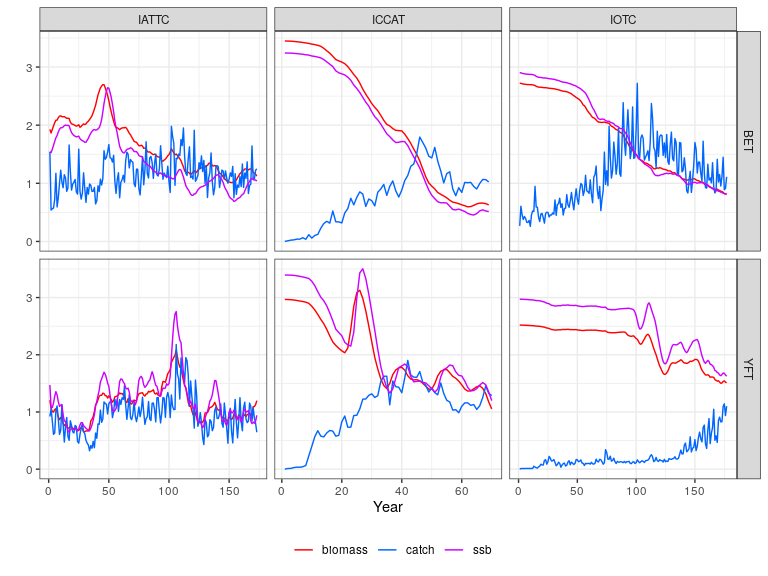
\includegraphics[width=\textwidth]{pe-tsmsy-1.png}
\caption{Time series of SSB (blue), biomass (red?) and fishing mortality (purple) relative to $MSY$ based reference points.}
\label{fig:ts}
\end{figure}


\newpage
\begin{figure}[h]
\centering
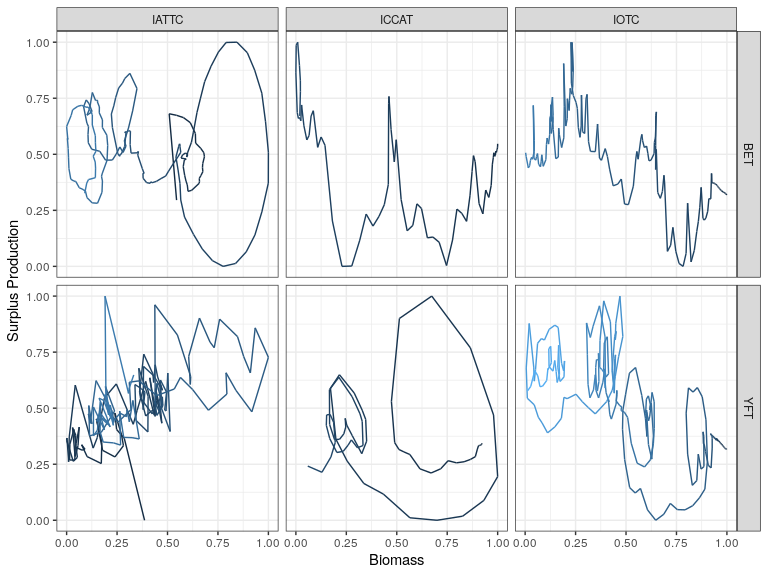
\includegraphics[width=\textwidth]{pe-sp2-1.png}
\caption{Surplus production plotted against biomass, dark to light trajectory colours indicates early to late period; clockwise loops in surplus production indicate positive production anomalies.}
\label{fig:sp}
\end{figure}


\newpage
\begin{figure}[h]
\centering
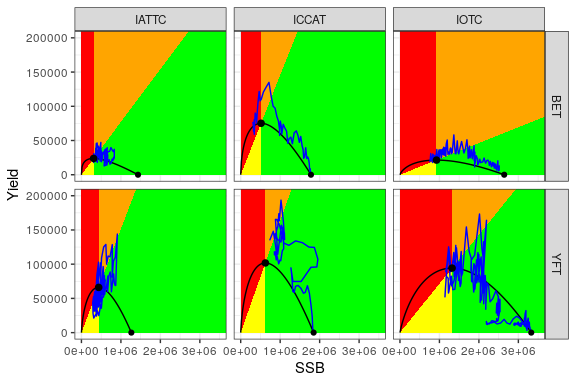
\includegraphics[width=\textwidth]{pe-pf2-1.png}
\caption{Surplus Production phase plots, with trajectories of catch and biomass; coloured regions correspond to Kobe quadrants, i.e. red indicates overfishing and overfished corresponding to the Kobe phase plot classification.}
\label{fig:pf}
\end{figure}


\newpage
\begin{figure}[h]
\centering
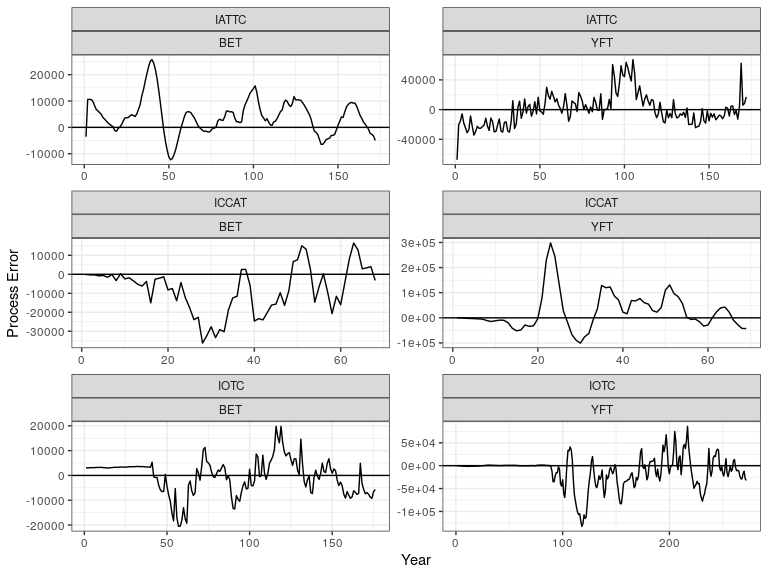
\includegraphics[width=\textwidth]{pe-pe-1.png}
\caption{Time series of process error expressed deviation of stochastic biomass and its deterministic expectation for time step}.
\label{fig:pe}
\end{figure}


\newpage
\begin{figure}[h]
\centering
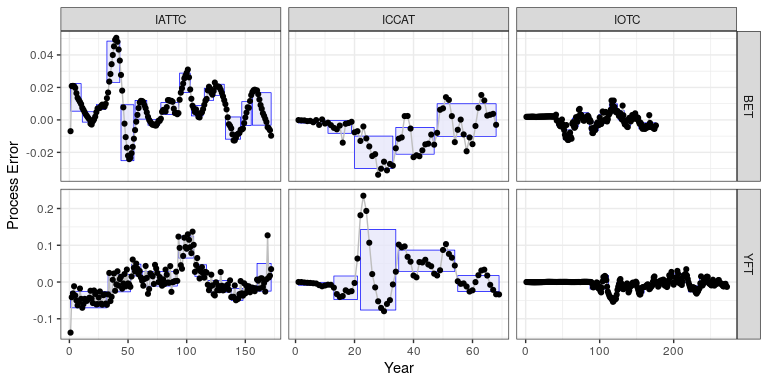
\includegraphics[width=\textwidth]{pe-pe2-1.png}
\caption{Process error, scaled relative to mean biomass, with regimes.}
\label{fig:pe2}
\end{figure}


\end{document}

Update B-ratio and/or F-ratio values from recent assessments and deal with F0.1 issue.

2. Retained Species: Assessed
2.1. Objective
Update B-ratio and/or F-ratio values from recent assessments and deal with F0.1 issue.


12. Environmental Pressure
12.1. Objective
Create an indicator based on impact of habit on fisheries



\clearpage
\section{Figures}


\newpage
\begin{figure}[h]
\centering
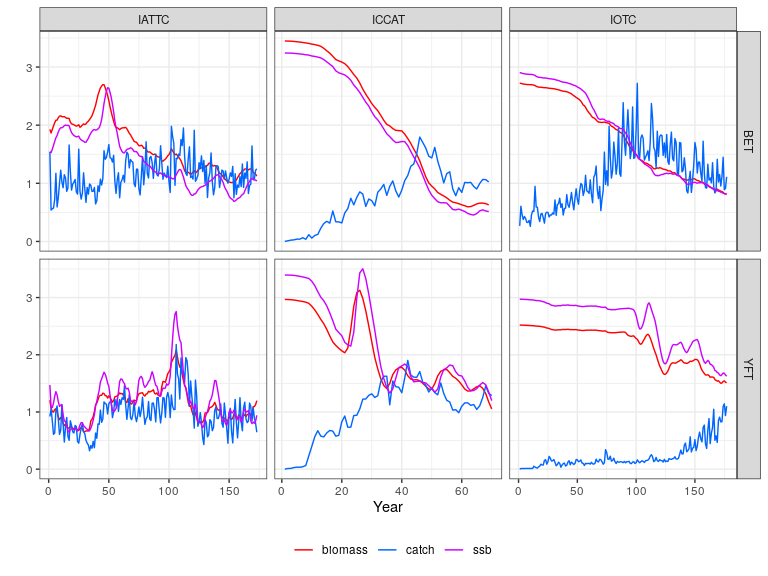
\includegraphics[width=\textwidth]{pe-tsmsy-1.png}
\caption{Time series of SSB (blue), biomass (red?) and fishing mortality (purple) relative to $MSY$ based reference points.}
\label{fig:ts}
\end{figure}


\newpage
\begin{figure}[h]
\centering
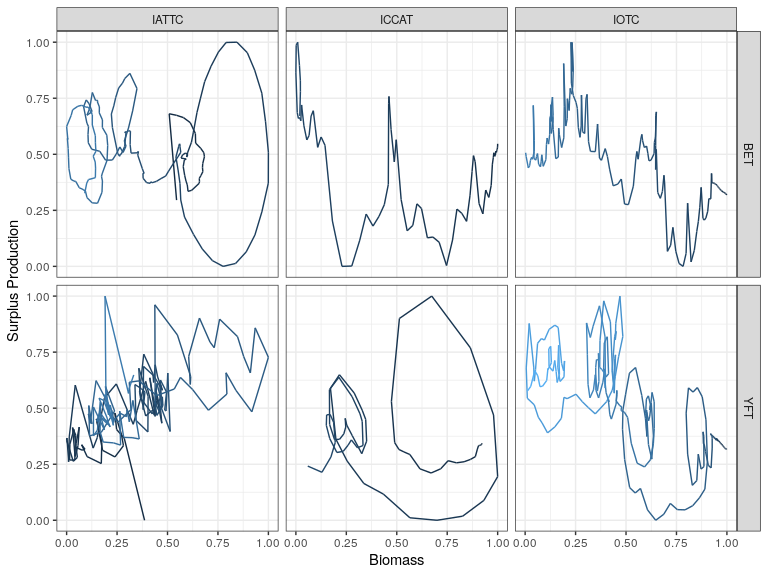
\includegraphics[width=\textwidth]{pe-sp2-1.png}
\caption{Surplus production plotted against biomass, dark to light trajectory colours indicates early to late period; clockwise loops in surplus production indicate positive production anomalies.}
\label{fig:sp}
\end{figure}


\newpage
\begin{figure}[h]
\centering
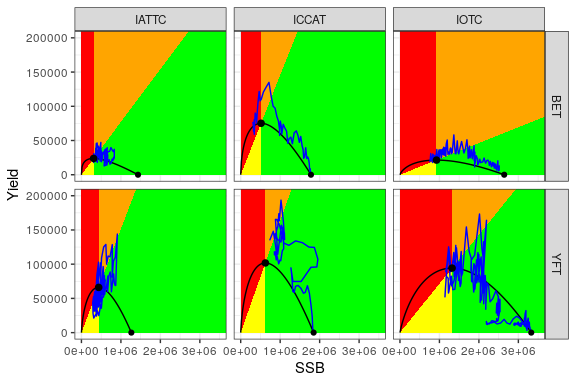
\includegraphics[width=\textwidth]{pe-pf2-1.png}
\caption{Surplus Production phase plots, with trajectories of catch and biomass; coloured regions correspond to Kobe quadrants, i.e. red indicates overfishing and overfished corresponding to the Kobe phase plot classification.}
\label{fig:pf}
\end{figure}


\newpage
\begin{figure}[h]
\centering
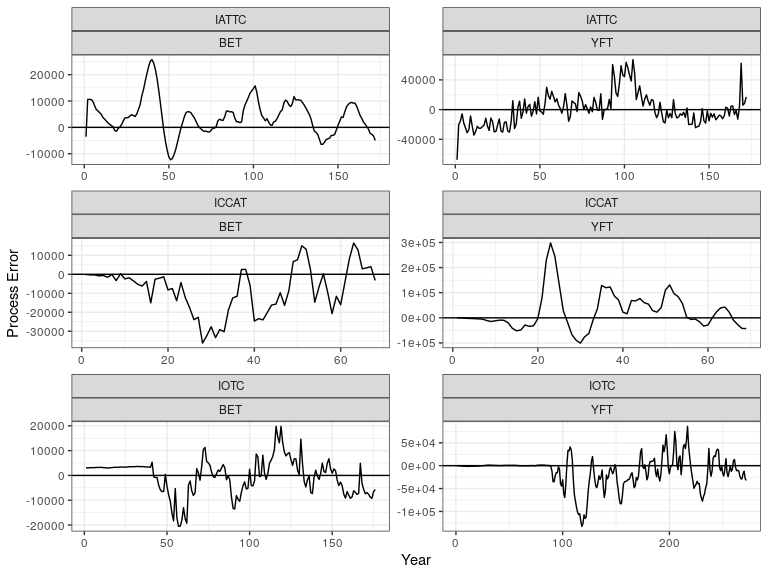
\includegraphics[width=\textwidth]{pe-pe-1.png}
\caption{Time series of process error expressed deviation of stochastic biomass and its deterministic expectation for time step}.
\label{fig:pe}
\end{figure}


\newpage
\begin{figure}[h]
\centering
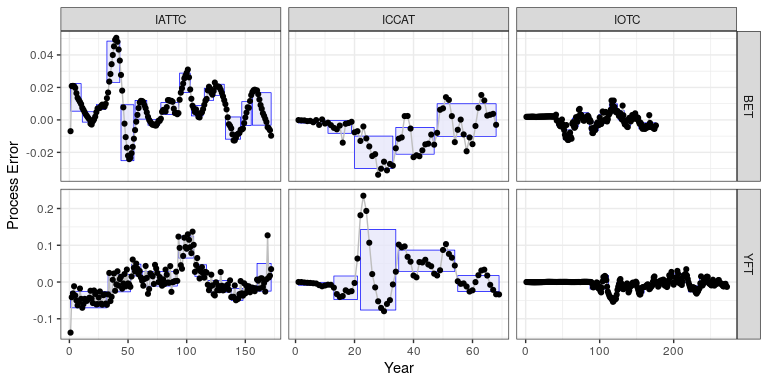
\includegraphics[width=\textwidth]{pe-pe2-1.png}
\caption{Process error, scaled relative to mean biomass, with regimes.}
\label{fig:pe2}
\end{figure}


\end{document}

Update B-ratio and/or F-ratio values from recent assessments and deal with F0.1 issue.

2. Retained Species: Assessed
2.1. Objective
Update B-ratio and/or F-ratio values from recent assessments and deal with F0.1 issue.


12. Environmental Pressure
12.1. Objective
Create an indicator based on impact of habit on fisheries



\clearpage
\section{Figures}


\newpage
\begin{figure}[h]
\centering
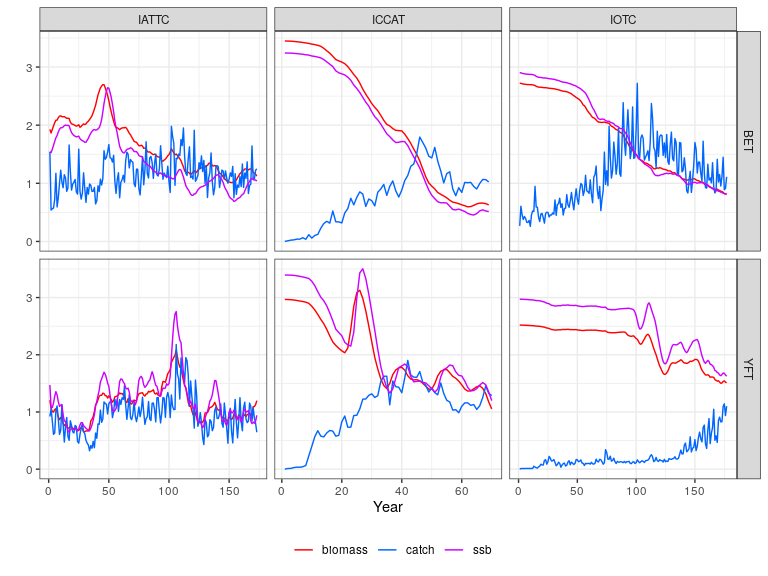
\includegraphics[width=\textwidth]{pe-tsmsy-1.png}
\caption{Time series of SSB (blue), biomass (red?) and fishing mortality (purple) relative to $MSY$ based reference points.}
\label{fig:ts}
\end{figure}


\newpage
\begin{figure}[h]
\centering
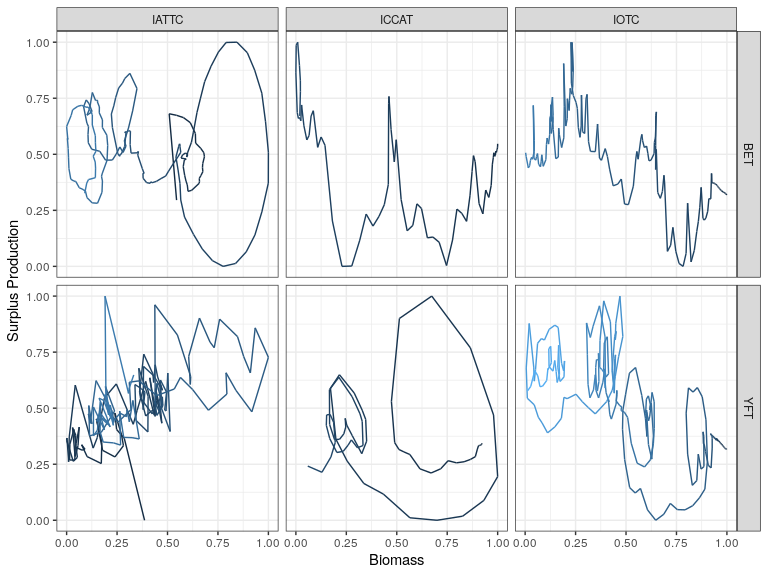
\includegraphics[width=\textwidth]{pe-sp2-1.png}
\caption{Surplus production plotted against biomass, dark to light trajectory colours indicates early to late period; clockwise loops in surplus production indicate positive production anomalies.}
\label{fig:sp}
\end{figure}


\newpage
\begin{figure}[h]
\centering
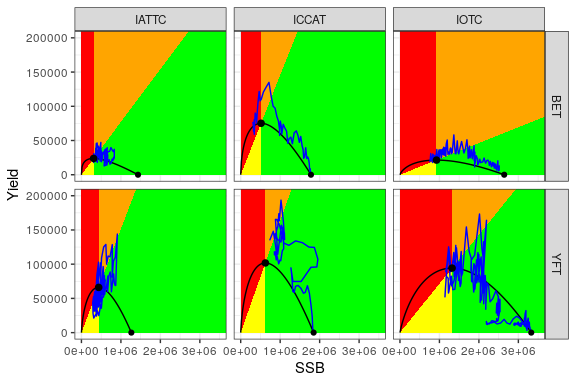
\includegraphics[width=\textwidth]{pe-pf2-1.png}
\caption{Surplus Production phase plots, with trajectories of catch and biomass; coloured regions correspond to Kobe quadrants, i.e. red indicates overfishing and overfished corresponding to the Kobe phase plot classification.}
\label{fig:pf}
\end{figure}


\newpage
\begin{figure}[h]
\centering
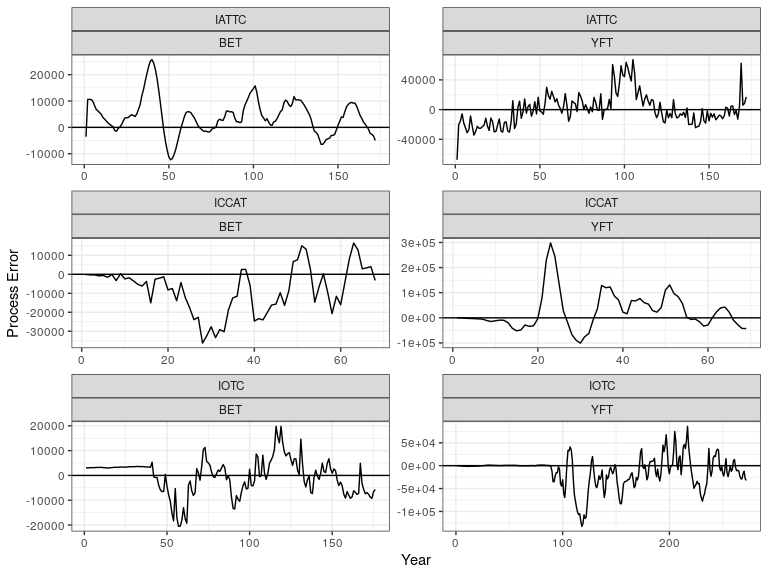
\includegraphics[width=\textwidth]{pe-pe-1.png}
\caption{Time series of process error expressed deviation of stochastic biomass and its deterministic expectation for time step}.
\label{fig:pe}
\end{figure}


\newpage
\begin{figure}[h]
\centering
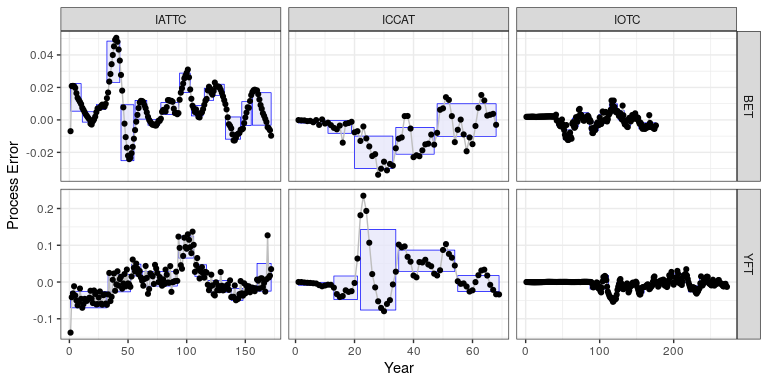
\includegraphics[width=\textwidth]{pe-pe2-1.png}
\caption{Process error, scaled relative to mean biomass, with regimes.}
\label{fig:pe2}
\end{figure}


\end{document}

Update B-ratio and/or F-ratio values from recent assessments and deal with F0.1 issue.

2. Retained Species: Assessed
2.1. Objective
Update B-ratio and/or F-ratio values from recent assessments and deal with F0.1 issue.


12. Environmental Pressure
12.1. Objective
Create an indicator based on impact of habit on fisheries



\clearpage
\section{Figures}


\newpage
\begin{figure}[h]
\centering
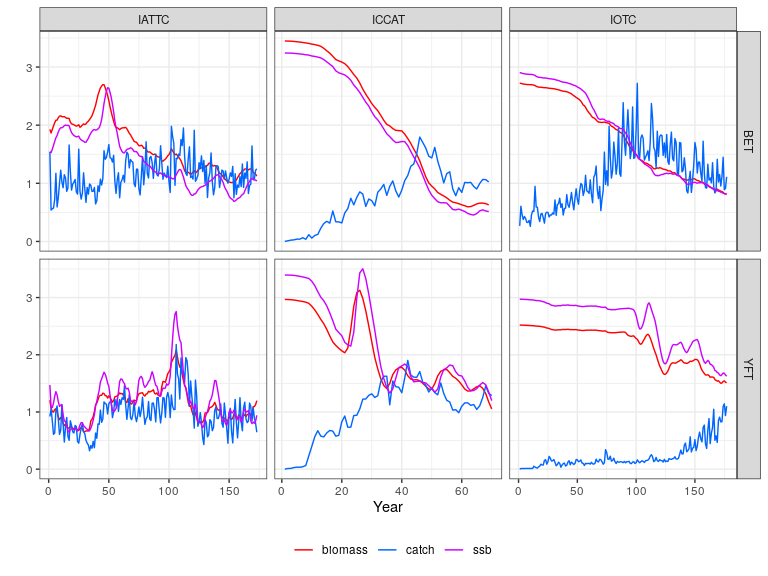
\includegraphics[width=\textwidth]{pe-tsmsy-1.png}
\caption{Time series of SSB (blue), biomass (red?) and fishing mortality (purple) relative to $MSY$ based reference points.}
\label{fig:ts}
\end{figure}


\newpage
\begin{figure}[h]
\centering
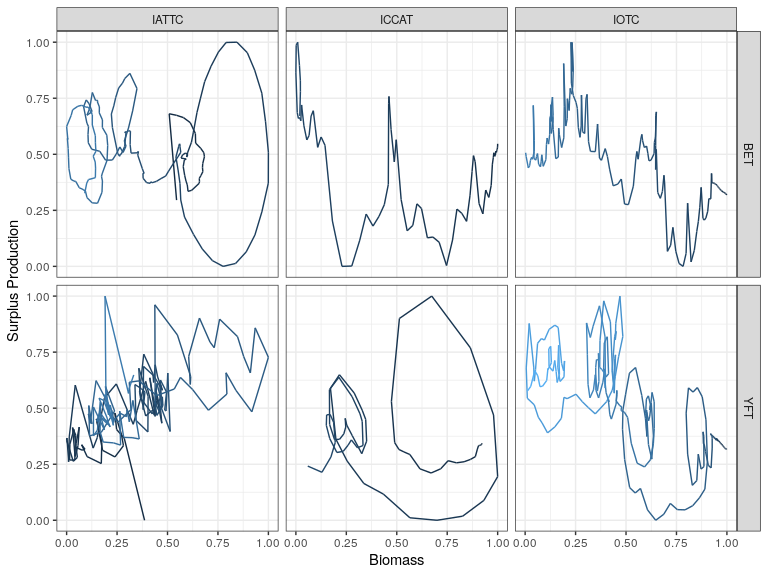
\includegraphics[width=\textwidth]{pe-sp2-1.png}
\caption{Surplus production plotted against biomass, dark to light trajectory colours indicates early to late period; clockwise loops in surplus production indicate positive production anomalies.}
\label{fig:sp}
\end{figure}


\newpage
\begin{figure}[h]
\centering
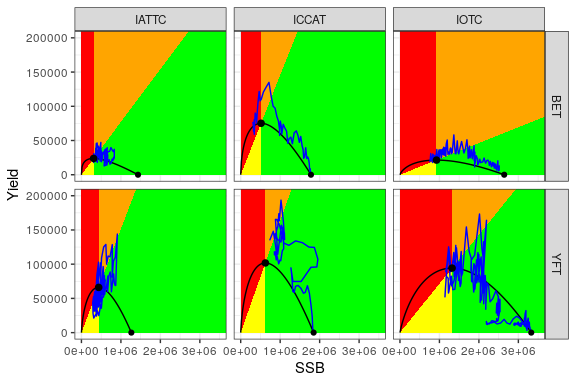
\includegraphics[width=\textwidth]{pe-pf2-1.png}
\caption{Surplus Production phase plots, with trajectories of catch and biomass; coloured regions correspond to Kobe quadrants, i.e. red indicates overfishing and overfished corresponding to the Kobe phase plot classification.}
\label{fig:pf}
\end{figure}


\newpage
\begin{figure}[h]
\centering
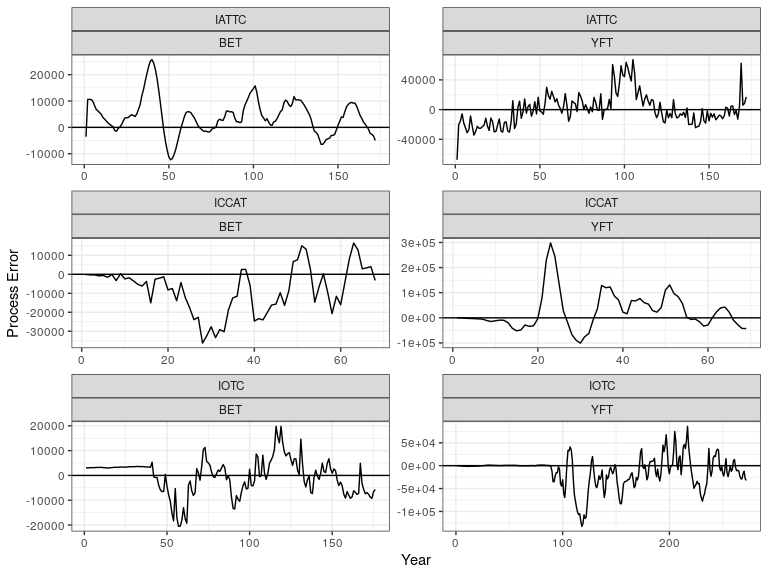
\includegraphics[width=\textwidth]{pe-pe-1.png}
\caption{Time series of process error expressed deviation of stochastic biomass and its deterministic expectation for time step}.
\label{fig:pe}
\end{figure}


\newpage
\begin{figure}[h]
\centering
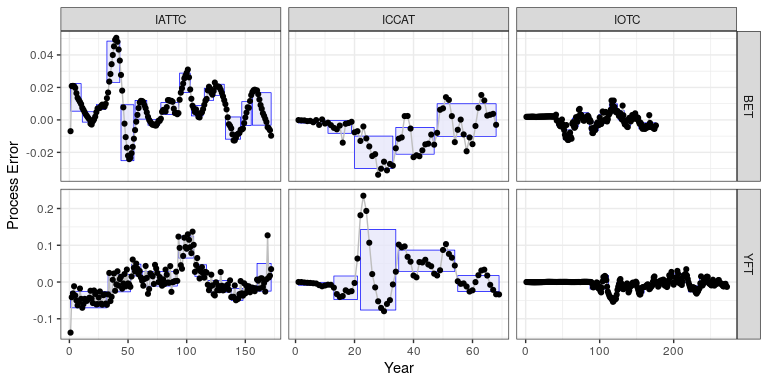
\includegraphics[width=\textwidth]{pe-pe2-1.png}
\caption{Process error, scaled relative to mean biomass, with regimes.}
\label{fig:pe2}
\end{figure}


\end{document}

Update B-ratio and/or F-ratio values from recent assessments and deal with F0.1 issue.

2. Retained Species: Assessed
2.1. Objective
Update B-ratio and/or F-ratio values from recent assessments and deal with F0.1 issue.


12. Environmental Pressure
12.1. Objective
Create an indicator based on impact of habit on fisheries

